\documentclass{minimal}
\usepackage{tikz}
\usetikzlibrary{shapes.gates.logic.US,trees,positioning,arrows}
\begin{document}
	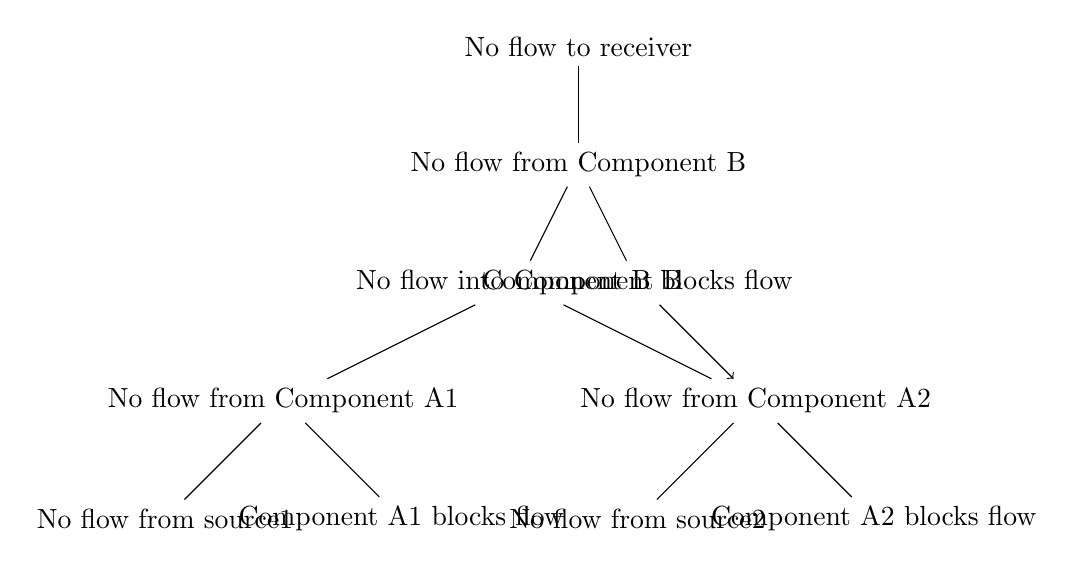
\begin{tikzpicture}[
	% Event style
	event/.style={rectangle}%,thick,draw,fill=yellow!20,text width=2cm, text centered,font=\sffamily,anchor=north},
	% Children and edges style
	%edge from parent/.style={very thick,draw=black!70},
	%edge from parent path={(\tikzparentnode.south) -- ++(0,-1.05cm)	-| (\tikzchildnode.north)},
	%level 1/.style={sibling distance=7cm,level distance=1.4cm,growth parent anchor=south,nodes=event},
	level 2/.style={sibling distance=7cm},
	level 3/.style={sibling distance=6cm},
	level 4/.style={sibling distance=3cm}
	]
	%% Draw events and edges
	\node (g1) [event] {No flow to receiver}
	child{node (g2) {No flow from Component B}   
		child {node (g3) {No flow into Component B}
			child {node (g4) {No flow from Component A1}
				child {node (t1) {No flow from source1}}
				child {node (b2) {Component A1 blocks flow}}
			}
			child {node (g5) {No flow from Component A2}
				child {node (t2) {No flow from source2}}
				child {node (b3) {Component A2 blocks flow}}
			}
		}
		child {node (b1) {Component B blocks flow}}
	};
	\draw [<-] (g5) -- (b1);
	\end{tikzpicture}
\end{document}
